\chapter{Evaluation}
\label{cha:results}

\section{Evaluation Tools}
Conducting a comprehensive performance evaluation of parallel algorithms across multiple High-Performance Computing (HPC) systems presents significant logistical challenges. Each system may have a different architecture, operating environment, and job scheduler configuration. Ensuring that experiments are run consistently, and that results are collected in a structured and reproducible manner, is essential for producing an accurate evaluation. To address these challenges, this work utilized SbatchMan, a Python-based command-line tool designed to automate and manage the submission of batch jobs to HPC clusters running the Slurm Workload Manager and the PBS Workload Manager. The tool is open-source and is available on GitHub\footnote{\url{https://github.com/LorenzoPichetti/SbatchMan}}. The tool was developed as a joint effort by the author and the thesis co-supervisor, Thomas Pasquali.

\subsection{SBatchMan design philosophy}

The core design philosophy of SbatchMan is the explicit separation of the execution environment from the experimental logic. This is a powerful abstraction that allows the same set of experiments to be deployed across different HPC clusters with minimal changes. This decoupling is achieved through two distinct types of configuration files, both written in the human-readable YAML format.

\begin{itemize}
    \item Cluster Configuration File: This file defines the hardware and scheduler specifics of a target machine. It contains all the environment-dependent directives, such as the cluster type (e.g., Slurm, PBS, or a local Linux machine), the target partition or queue, the requested number of nodes, CPUs per task, and the wall-clock time limit. By encapsulating these details, the cluster configuration file acts as a reusable profile for a specific HPC system.
    \item Job Configuration File: This file defines the actual suite of experiments to be run. It references a specific cluster configuration to determine where the jobs will run, but its primary focus is on what to run. This includes the command template for the executable and, most importantly, a powerful variable system for defining the parameter space of the experiments. The user can define a matrix of variables, such as a list of input graph files or a range of thread counts. SbatchMan automatically computes the Cartesian product of all specified variables, generating a unique job for every possible combination. This file also allows for the setting of environment variables and the definition of pre-execution or post-execution commands, providing full control over the job's lifecycle.
\end{itemize}
    
In the context of this thesis, SbatchMan was used to conduct the evaluation of the OpenMP and the pthreads-based BFS implementation. It was used to systematically vary the number of threads, the input graph datasets and the implementations' configuration parameters. By using a single job configuration file and multiple cluster-specific files, SbatchMan ensured that the evaluation conditions were identical across all runs on all target systems, thereby eliminating a significant source of potential experimental error.

\subsection{Other tools}
To facilitate the efficient loading of graph data, both implementations utilize the \texttt{distributed\_mmio} library\footnote{\url{https://github.com/HicrestLaboratory/distributed\_mmio}}. This C++ library provides a simple and high-performance interface for reading and parsing matrices stored in the Matrix Market (.mtx) file format. Many common benchmark graphs, such as those from collections like the SuiteSparse Matrix Collection\footnote{\url{https://sparse.tamu.edu/}}, are available in this format, simplifying the process of importing real-world data for evaluation. The library is designed for efficiency, capable of quickly parsing large graph files into a memory-efficient representation. To enable its use in the C-based pthreads implementation, a C wrapper was developed as a contribution to the project, exposing the core C++ parsing functionality through a C-compatible API.

The acquisition and generation of graph datasets for the evaluation were managed using MtxMan\footnote{\url{https://github.com/ThomasPasquali/MtxMan}}, a command-line tool designed to streamline graph data management. This tool simplifies the process of downloading and extracting graphs from the SuiteSparse Matrix Collection. Additionally, MtxMan includes generators for creating synthetic graphs with specific structural properties, which is valuable for testing algorithmic performance under controlled conditions.

\section{Evaluation Datasets}
The practical relevance of a Breadth-First Search algorithm extends beyond being a benchmark of computing power. The graphs chosen for evaluation in this work apply BFS as either a direct solution or a fundamental building block for solving real-world problems. Given that the MergedCSR structure adapts well only to graphs with smaller frontiers, the selection of graphs classes was restricted to the ones that have a consistent frontier size (see \cref{fig:frontiersize}). The selected graphs come from the following domains: Road Networks and Random Geometric Graphs (RGGs). The selected graphs are taken from the SuiteSparse Matrix Collection and their characteristics are summarized in \cref{tab:datasets_booktabs}.
\paragraph{Road networks} For road networks, the application of BFS is intuitive: it is the foundational algorithm for pathfinding and reachability analysis. In this context, vertices represent intersections and edges represent road segments \cite{thomson1995graph}. On these graphs, the BFS is applied to solve problems involving navigation, logistics, and emergency services.
\paragraph{Finite Element Models (FEM)} In the context of finite element analysis, vertices represent nodes in a physical mesh and edges represent the connections between them \cite{chen2018finite}. Here, BFS is used to model the propagation of physical phenomena. This is applied to perform stress and strain analysis and crack propagation simulations.
\paragraph{Random Geometric Graphs (RGGs)} Random geometric graphs serve as theoretical models for real-world networks where connectivity is determined by physical proximity \cite{penrose2003random}. For example, RGGs are used to model wireless networks, where nodes can only communicate with others within a certain range or for epidemiology and contagion modeling in a population, since the spread of a disease occurs through close contact among individuals \cite{kenniche2010random, estrada2016epidemic}.

\begin{table}[h]
    \centering
    \begin{tabularx}{\linewidth}{ l l c c l }
    \toprule
    \multicolumn{1}{c}{\textbf{Name}} & \multicolumn{1}{c}{\textbf{Graph class}} & \multicolumn{1}{c}{\textbf{Vertices}} &
    \multicolumn{1}{c}{\textbf{Edges}} & 
    \multicolumn{1}{c}{\textbf{Notes}}\\
    \midrule
    GAP-Road      & Road Network & 23.9M & 57.7M & Road network of the USA. \\
    europe\_osm   & Road Network & 50.9M & 108M  & Road network of Europe. \\
    asia\_osm     & Road Network & 11.9M & 25.4M & Road network of Asia. \\
    \addlinespace % Adds a little extra space for visual separation
    Geo\_1438     & FEM          & 1.4M  & 60.2M & Geomechanical model of Earth's crust. \\
    Hook\_1498    & FEM          & 1.4M  & 59.4M & 3D model of a steel hook. \\
    PFlow\_742     & FEM          & 0.7M  & 37.1M & 3D pressure-temp in porous media. \\
    \addlinespace % Adds a little extra space for visual separation
    rgg\_n\_2\_22\_s0 & RGG          & 4.2M  & 60.7M & Random Geometric Graph. \\
    \bottomrule
    \end{tabularx}
    \caption{Datasets used in the evaluation.}
    \label{tab:datasets_booktabs}
\end{table}


\section{Evaluation Environment}
The C++/OpenMP implementation presented in \cref{sec:mergedcsr} and the C/pthreads implementation presented in \cref{sec:pthreads} are compared against the BFS implementation from the GAP benchmark. The evaluation was conducted on the following platforms:
\begin{itemize}
    \item \amd{}: AMD EPYC 7543 CPU @ 2.8 GHz (32 cores), with 32 KiB L1d cache, 32 KiB L1i cache and 512 KiB L2 cache per core, 256 MiB shared L3 cache, and 32 GB DDR4 RAM @ 3.2 GHz, nominal TDP 225W;
    \vspace{-2mm}
    \item \pioneer{} board: Sophon SG2042 RISC-V CPU @ 2.0 GHz (64 cores), with 64 KiB L1d cache and 64 KiB L1i cache per core, 1 MiB L2 cache shared per 4-core cluster, 64 MiB shared L3 cache, and 128 GB DDR4 RAM, nominal TDP 120W \cite{brown2023performance};
    \vspace{-2mm}
    \item \grace{}: NVIDIA Grace CPU Superchip @ up to 3.0 GHz (144 cores), with 64 KiB L1d cache, 64 KiB L1i cache and 1 MiB L2 cache per core, 228 MiB shared L3 cache, and 960 GB LPDDR5X RAM, nominal TDP 500W (including memory) \cite{elster2022nvidia}.
    \vspace{-2mm}
\end{itemize}
For each dataset, performance was measured by starting the BFS from 32 random source vertices, with the first two runs discarded to mitigate warm-up effects. The geometric mean of the subsequent runtimes was taken as the final metric for each graph. When aggregating results, the geometric mean of these individual metrics was used to represent the performance for each graph class.

\section{Results}
This section presents a comparative performance evaluation of the two parallel BFS implementations developed in this thesis: the cache-optimized OpenMP version from \cref{sec:mergedcsr} (hereafter \openmp{}) and the explicit pthreads version from \cref{sec:pthreads} (hereafter \pthreads{}). To contextualize their performance, these two approaches are benchmarked against the BFS kernel from the GAP Benchmark Suite (\gapbs{}). The \gapbs{} implementation serves as a widely recognized baseline, providing a standard point of comparison common in graph analytics literature. The implemented code along with reproducibility instructions is available at \url{https://github.com/sasso0101/thesis}.

The performance analyses presented in \crefrange{sec:chunksize}{sec:pthreadsperf} are conducted on the \amd{} platform. \cref{sec:otherplatforms} then provides a comparative evaluation, benchmarking the performance of the AMD platform against the RISC-V-based Pioneer board and the ARM-based NVIDIA Grace CPU.

\subsection{Evaluation of the optimal chunk size}
\label{sec:chunksize}
The \chunksize{} is a key parameter in the pthreads implementation, defining the granularity of the work partitioning and load balancing system. A sensitivity analysis was conducted to find an optimal value, testing sizes from 4 to 1024. The results, shown in \cref{fig:chunksize}, reveal that the optimal granularity is highly dependent on the degree of parallelism.

In the single-threaded case, where no parallel work-stealing occurs, performance is dictated by the overhead of the chunking mechanism, with larger chunk sizes often proving more efficient. As the thread count increases, a clear trade-off between management overhead and load balancing effectiveness emerges. A \chunksize{} of 64, highlighted by the hatched bars, proves to be the most effective choice across the majority of multi-threaded scenarios. Smaller chunks increase the frequency of lock contention and queue management, while very large chunks minimize this overhead but provide too few opportunities for the work-stealing mechanism to effectively balance the load. Based on this analysis, a value of 1024 was used for single-threaded executions, while a value of 64 was used for all multi-threaded configurations in subsequent evaluations.

\subsection{Strong scaling analysis}
\label{sec:strongscaling}

\cref{fig:scaling_comparison} presents a strong scaling analysis of the \gapbs{}, \openmp{}, and \pthreads{} implementations. All three implementations exhibit effective strong scaling at lower core counts. However, their behavior diverges at 16 and 32 threads. The \gapbs{} and \openmp{} implementations, which share similar framework-based designs, show performance degradation, particularly on the large Road Network datasets. This negative scaling is likely due to the synchronization overhead overwhelming the computational work at high core counts. In contrast, the \pthreads{} implementation demonstrates more robust scaling, due to the lightweight barrier and dynamic work-stealing, which mitigates contention. The \texttt{asia\_osm} graph does not scale well because its frontier sizes are the smallest of the evaluated graphs (the \texttt{asia\_osm} graph has the lowest frontier size line in \cref{fig:frontiersize}), which limits the amount of parallelism that can be exploited.

\begin{figure}[h]
\centering
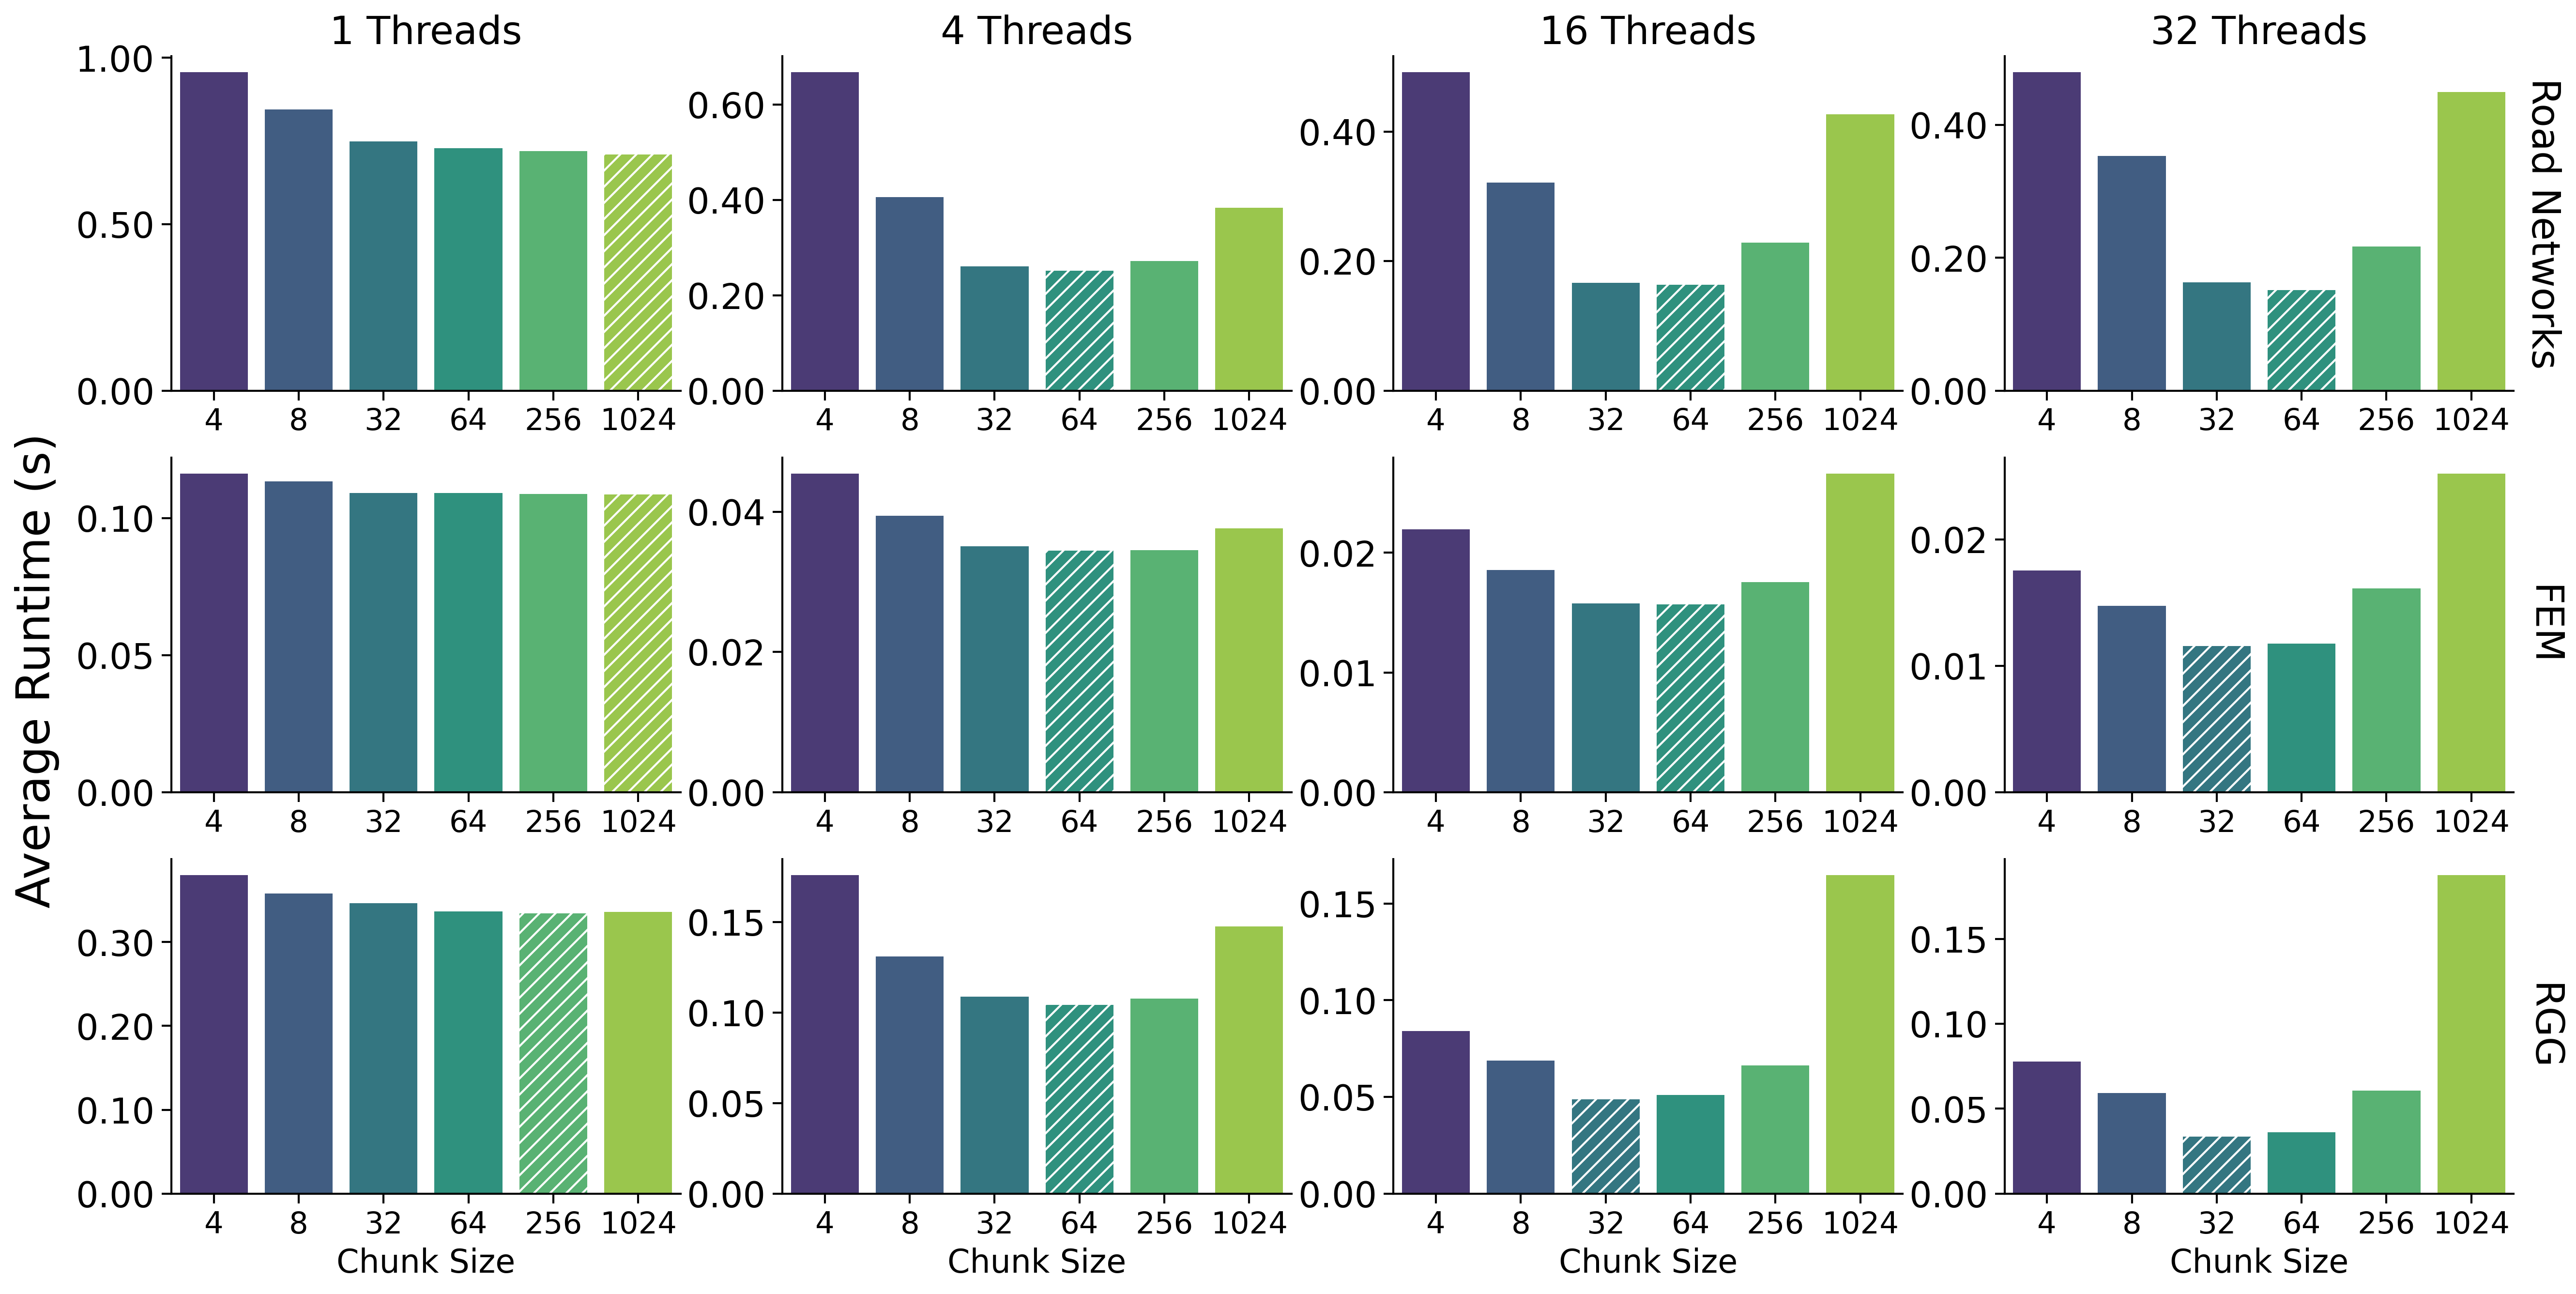
\includegraphics[width=\linewidth]{images/pthreads_chunksize.png}
\caption{Average runtime of the pthreads BFS implementation across various graph classes (rows), thread counts (columns), and \chunksize{} configurations (colored bars). The hatched bar in each subplot indicates the \chunksize{} that yielded the best performance for that specific configuration.}
\label{fig:chunksize}

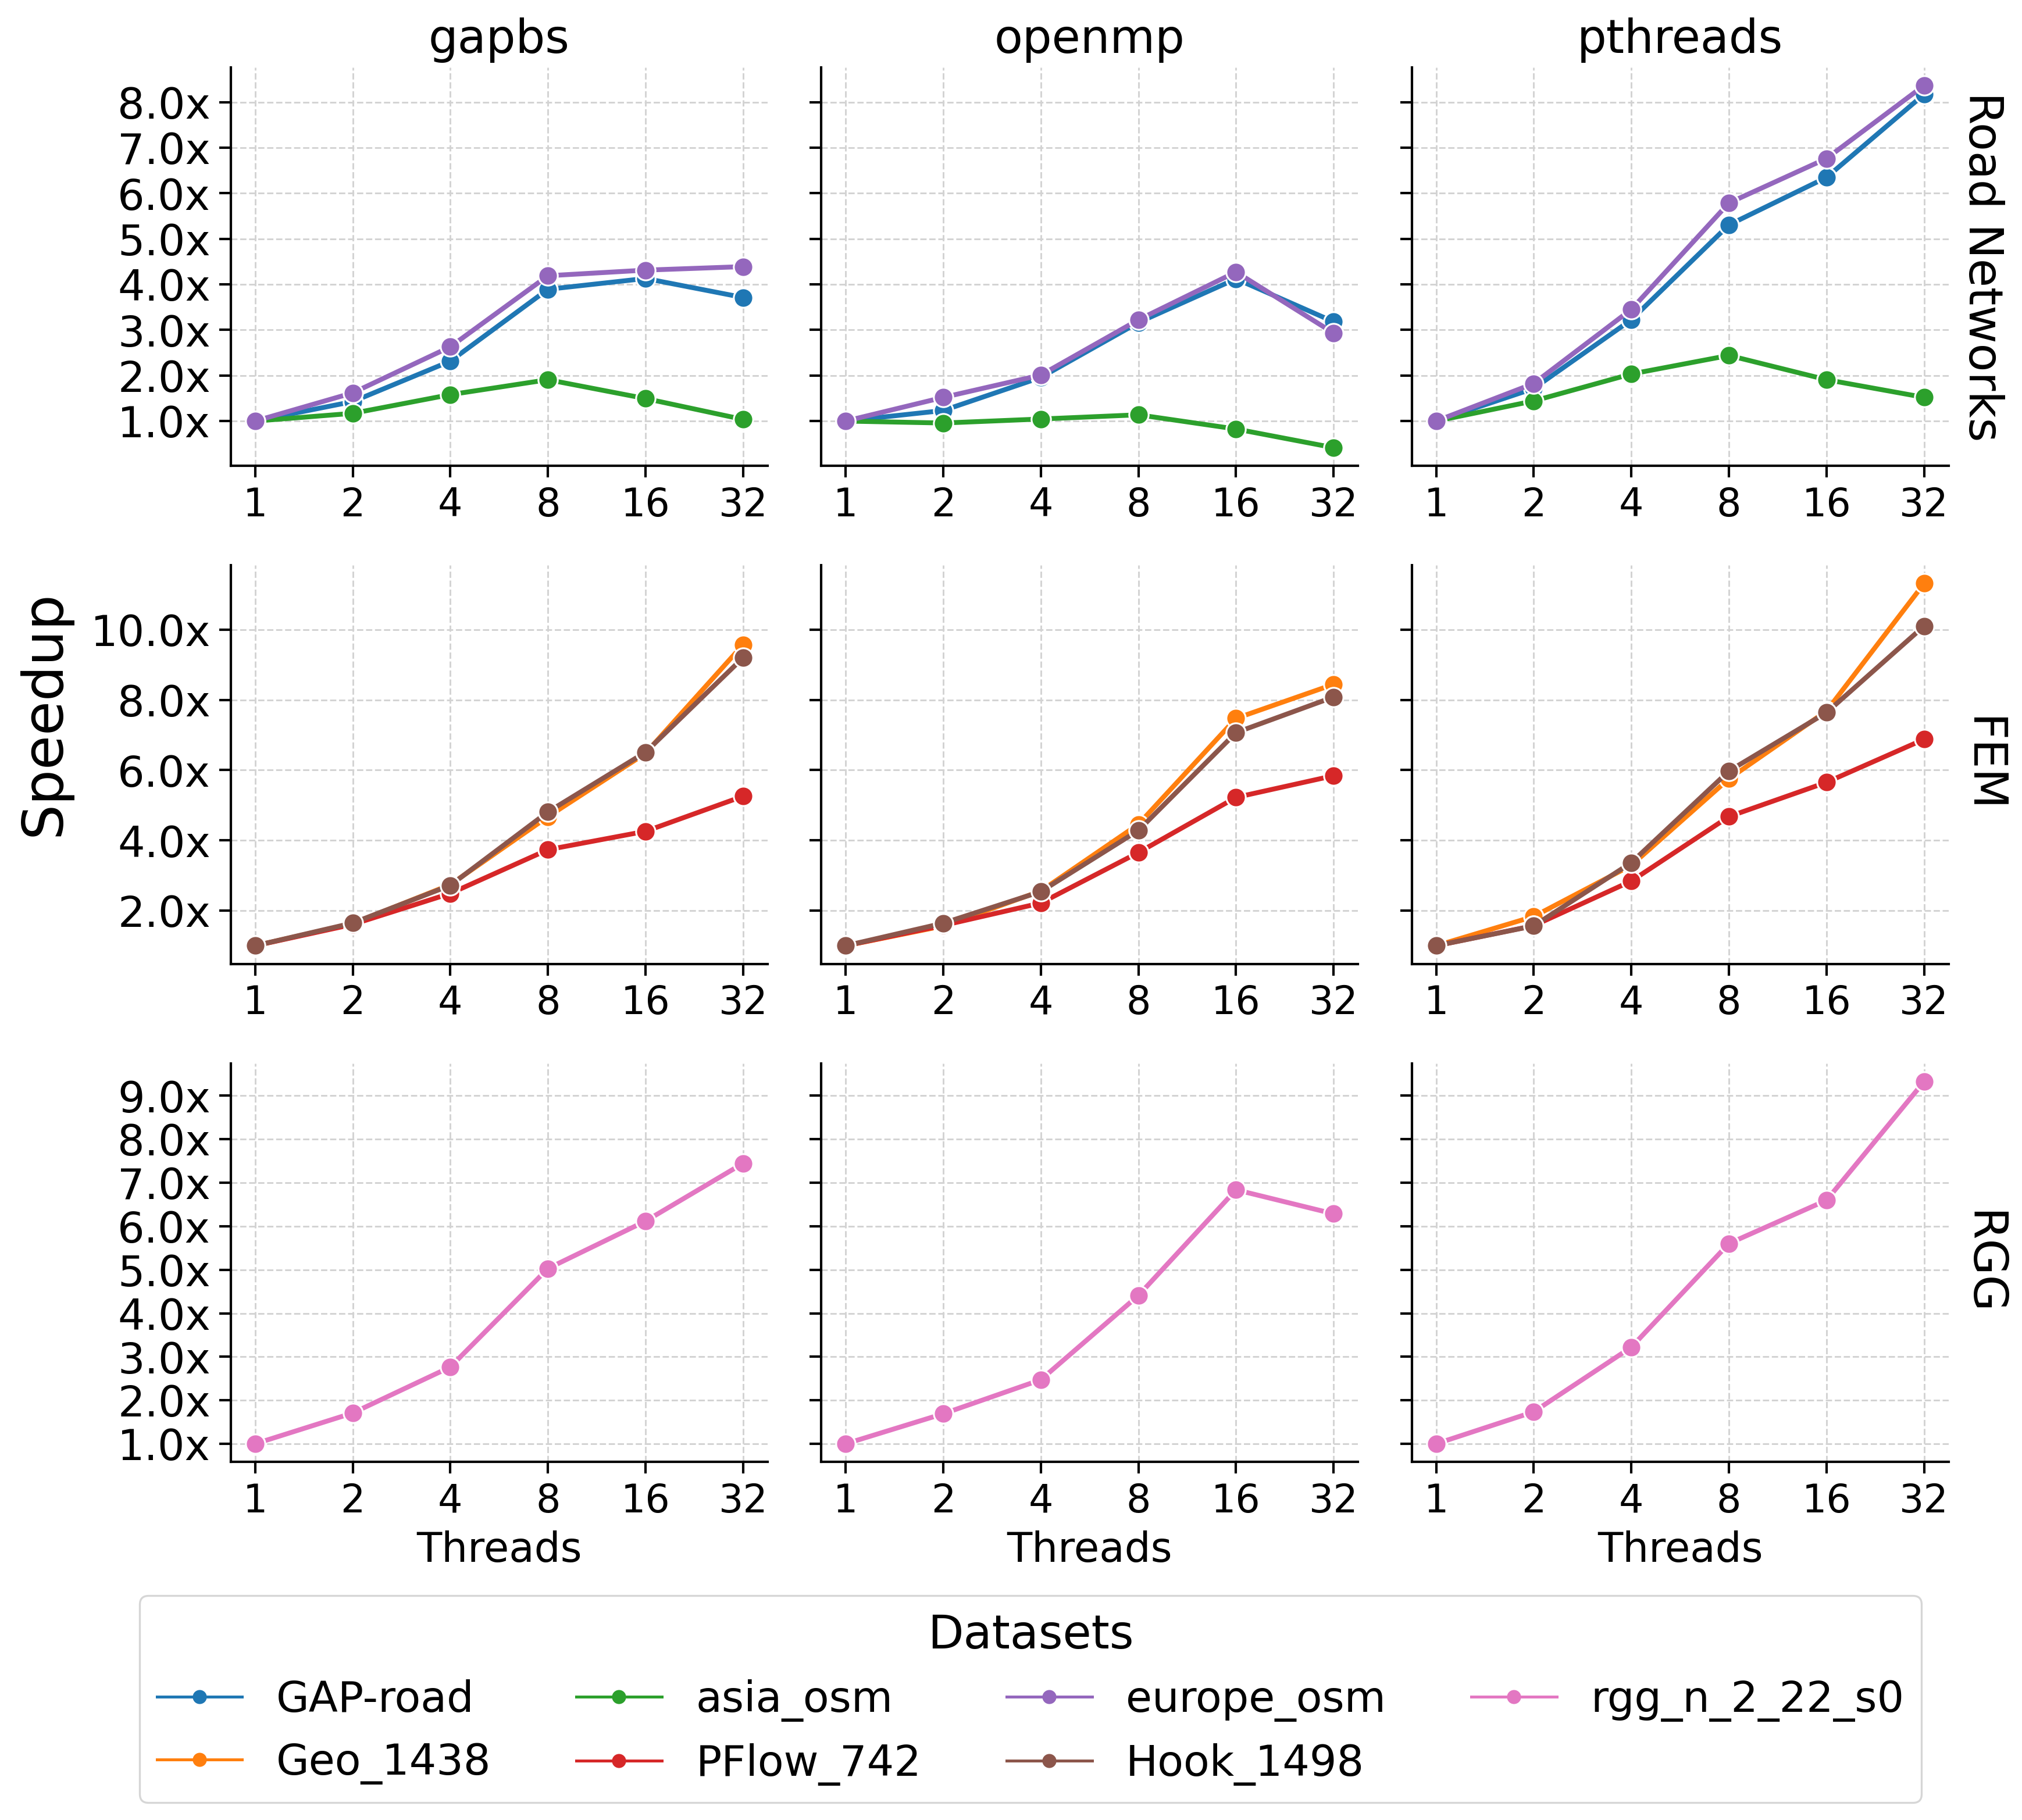
\includegraphics[width=0.8\linewidth]{images/scalability.png}
\caption{Scaling comparison of the evaluated implementations (columns) across various graph classes (rows). The plots show the speedup of each configuration as the number of CPU threads increases, relative to the one-threaded performance.}
\label{fig:scaling_comparison}
\end{figure}

\clearpage

\subsection{Performance of the MergedCSR implementation}
\label{sec:mergedcsrperf}

To quantify the performance impact of the cache-optimized MergedCSR data structure, the \openmp{} implementation was compared directly against the \gapbs{} baseline. \cref{fig:speedup_openmp} shows the speedup of the \openmp{} version relative to \gapbs{} across the three graph classes.

For the FEM graphs, the \openmp{} implementation is consistently slower than the \gapbs{} baseline, with a speedup below 1. The FEM graphs, while originating from mesh-based models, exhibit small-diameter characteristics such as rapid frontier growth. The \gapbs{} implementation, being direction-optimizing, detects this and leverages the more efficient Bottom-Up traversal strategy during the dense, intermediate phases of the search. For instance, on the \texttt{Hook\_1498} dataset, the Bottom-Up step is activated five times. In contrast, the \openmp{} implementation is restricted to a Top-Down-only traversal due to the design of its MergedCSR data structure. Consequently, it is at a significant algorithmic disadvantage on these specific graphs, as it is forced to use a less optimal strategy.

On the Road Networks and the RGG datasets, the frontiers instead remain small, and both \gapbs{} and \openmp{} exclusively use the Top-Down strategy. With the traversal algorithm being identical, the performance difference is now dictated by the efficiency of the underlying data structure. In this context, the benefits of the MergedCSR format are clearly visible. By improving spatial locality and reducing cache misses, the \openmp{} implementation significantly outperforms the baseline. This results in a geometric mean speedup of 1.47x on the Road Network datasets and 1.5x on the RGG dataset. This demonstrates that for workloads that are purely Top-Down, the cache-optimized data layout provides a substantial performance improvement over a standard CSR implementation.

\begin{figure}[h!]
\centering
% Assuming the image is saved as 'speedup_vs_gapbs.png' in the 'images' folder
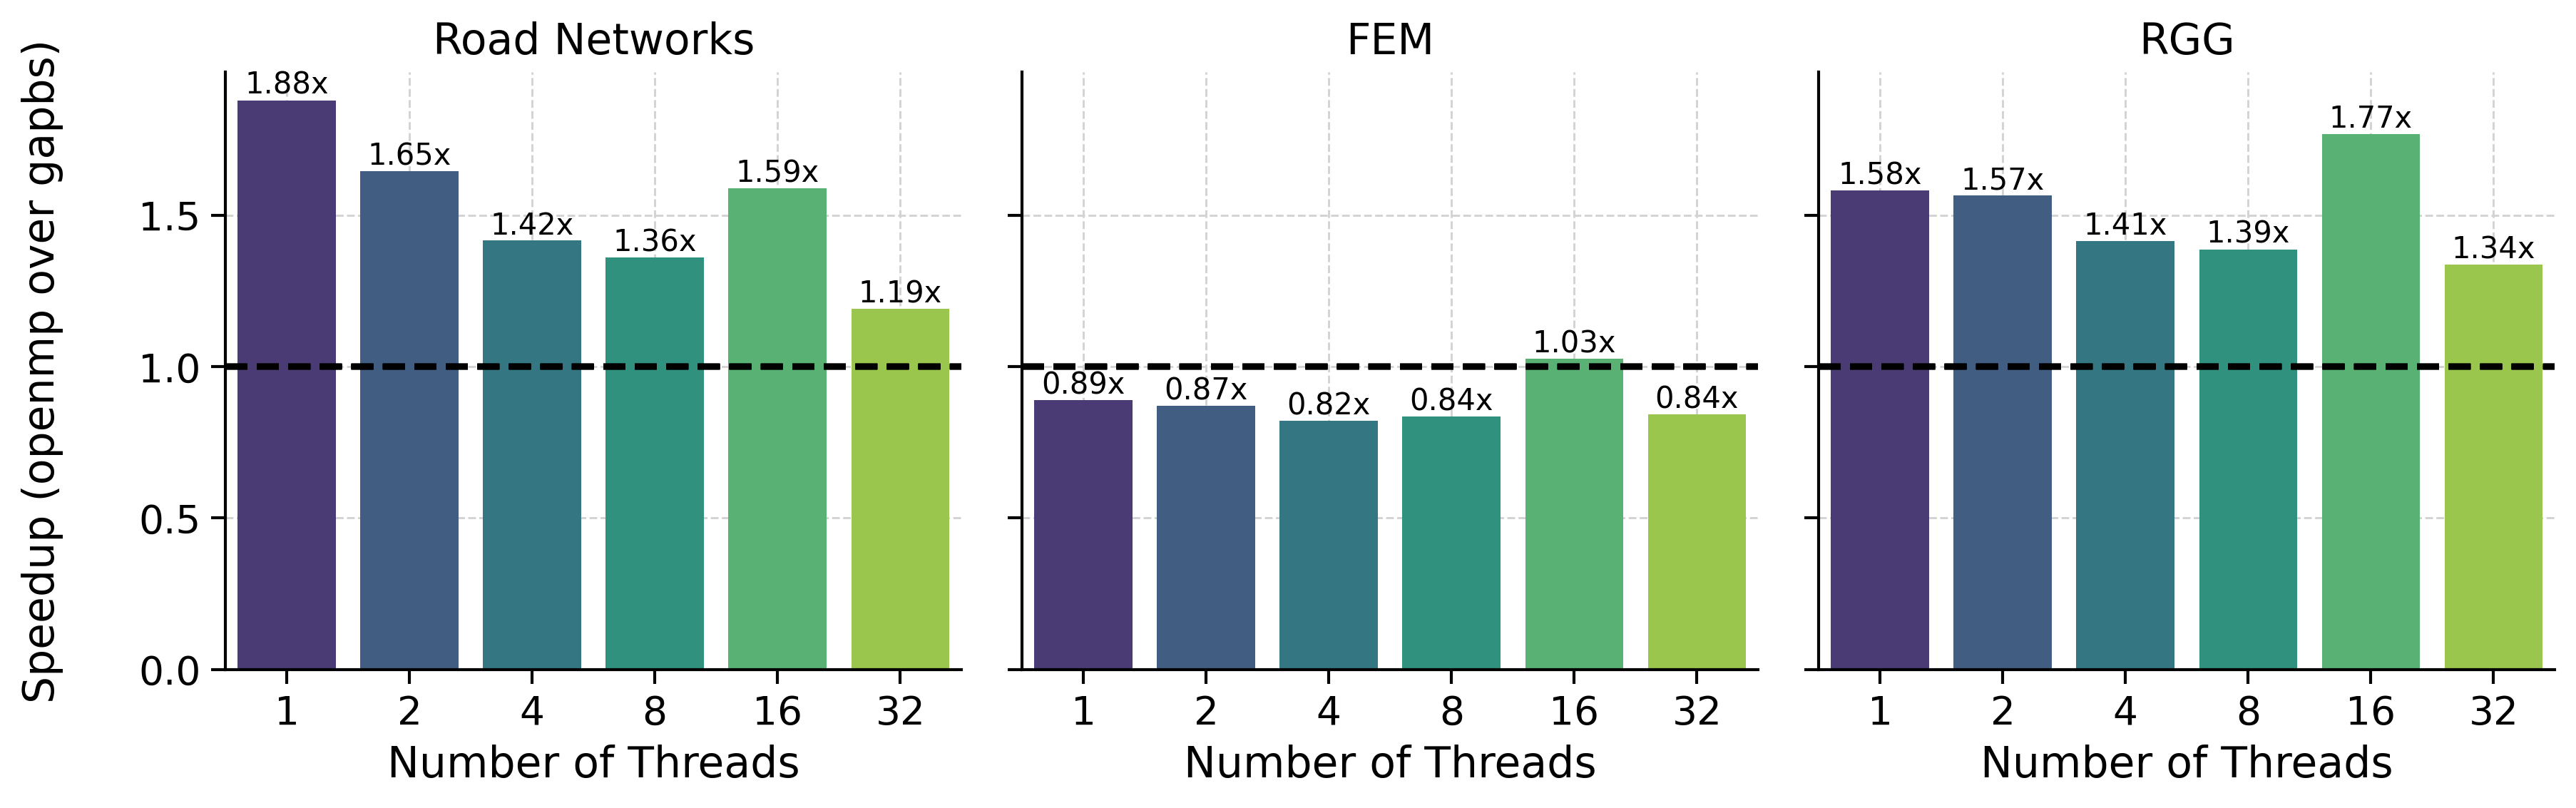
\includegraphics[width=\linewidth]{images/speedup_openmp.png}
\caption{Speedup of the \openmp{} implementation relative to the \gapbs{} baseline, grouped by graph class.}
\label{fig:speedup_openmp}
\end{figure}

\subsection{Performance of the pthreads implementation}
\label{sec:pthreadsperf}

To isolate the performance impact of the parallelization strategy, this section directly compares the explicit \pthreads{} implementation against the framework-based \openmp{} version. Both implementations utilize the same cache-optimized MergedCSR data structure, making this a direct comparison of their respective parallel execution models. \cref{fig:speedup_pthreads} illustrates the speedup of the \pthreads{} version relative to the \openmp{} implementation across the three graph classes.

The results again show a clear distinction in performance based on the graph type. On the FEM datasets, the performance of the \pthreads{} implementation is on par with the \openmp{} version. This is an expected outcome, as both implementations are constrained to a Top-Down-only traversal.

In contrast, on the large-diameter graphs where the Top-Down strategy is optimal, the benefits of the explicit \pthreads{} implementation become evident. The lightweight barrier and the dynamic work-stealing mechanism of the \pthreads{} version prove to be significantly more efficient and scalable than the general-purpose primitives provided by the OpenMP runtime. This results in a substantial performance advantage that grows with the number of threads, particularly visible at 32 threads for the Road Networks where the \pthreads{} version is nearly 2.8x faster. Quantitatively, this performance advantage translates to a geometric mean speedup of 1.55x for the \pthreads{} implementation across the Road Network datasets and 1.25x on the RGG dataset. Compared to the GAP benchmark, the achieved geomean speedup was 2.28x for the Road Network graphs (up to 3.6x for the \texttt{osm\_europe} graph) and 1.87x for the RGG dataset.

\begin{figure}[h!]
\centering
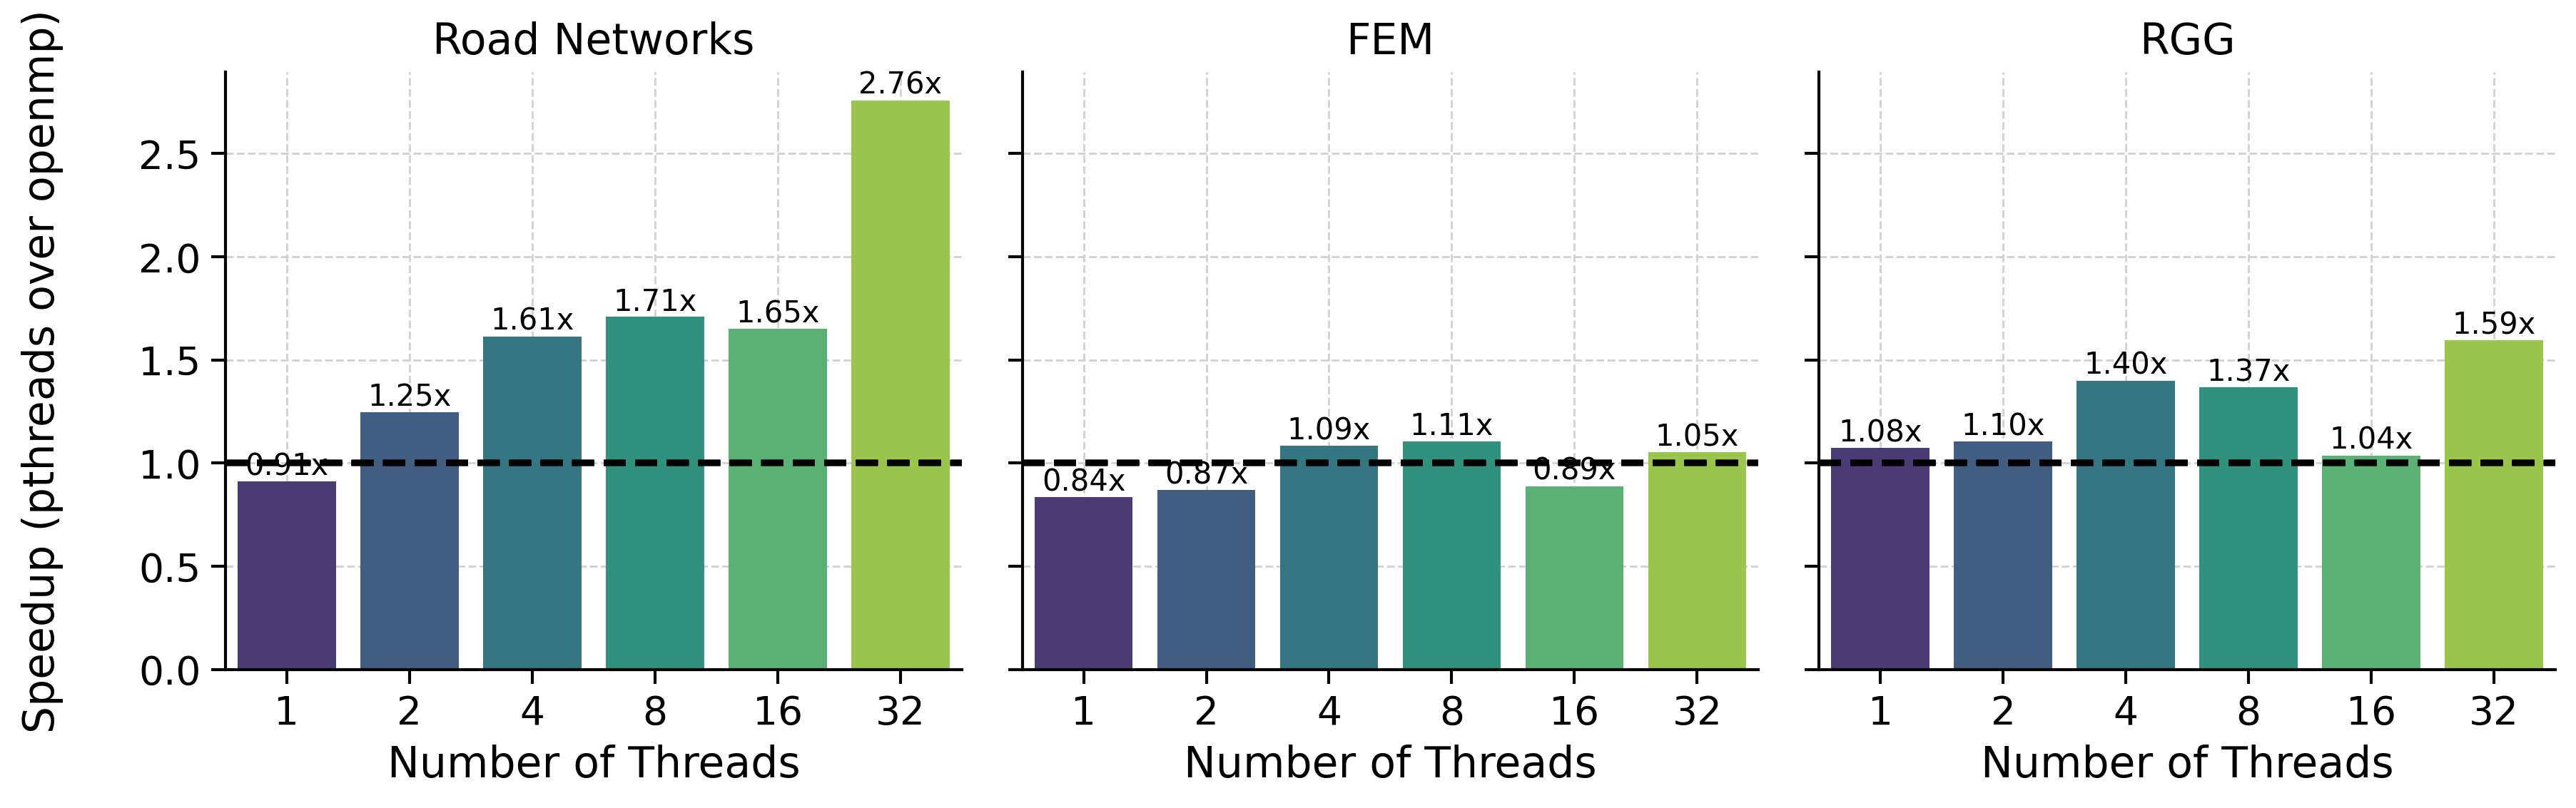
\includegraphics[width=0.95\linewidth]{images/speedup_pthreads.png}
\caption{Speedup of the \texttt{pthreads} implementation relative to the \texttt{openmp} implementation, grouped by graph class.}
\label{fig:speedup_pthreads}
\end{figure}

\subsection{Performance on diverse hardware platforms}
\label{sec:otherplatforms}

To provide a comprehensive analysis of the pthreads implementation's performance and portability, its strong scaling was evaluated on three distinct hardware platforms: the x86-based AMD EPYC, the ARM-based NVIDIA Grace CPU, and the RISC-V-based Sophon SG2042 (Pioneer board). The \texttt{europe\_osm} graph was selected for this comparison as it is the largest dataset evaluated, and the pthreads implementation was chosen as it demonstrated the most robust scaling in the previous analyses. Figure \cref{fig:platform_comparison} presents the absolute runtime and relative speedup for this configuration.

The results reveal significant architectural differences in both performance and scalability. The single-threaded performance is a direct reflection of each CPU's single-core processing power. The NVIDIA Grace and AMD EPYC CPUs exhibit comparable performance, with Grace being slightly faster. In contrast, the Pioneer board's RISC-V CPU is initially much slower, taking over 10 seconds. This is attributable to its lower clock frequency and lower Instructions Per Clock (IPC) compared to the more mature x86 and ARM server architectures. However, as the thread count increases, the Pioneer board's massive parallelism allows it to dramatically reduce its runtime achieving an almost linear speedup up to 8 threads, and a 15.2x speedup for 32 threads. The Grace and AMD CPUs exhibit similar performance up to 16 threads, but the Grace CPU's performance drops at 32 threads, likely due to the custom sense-reversal barrier's poor interaction with the cache coherence protocol of Grace's massively parallel architecture.

\begin{figure}[h!]
\centering
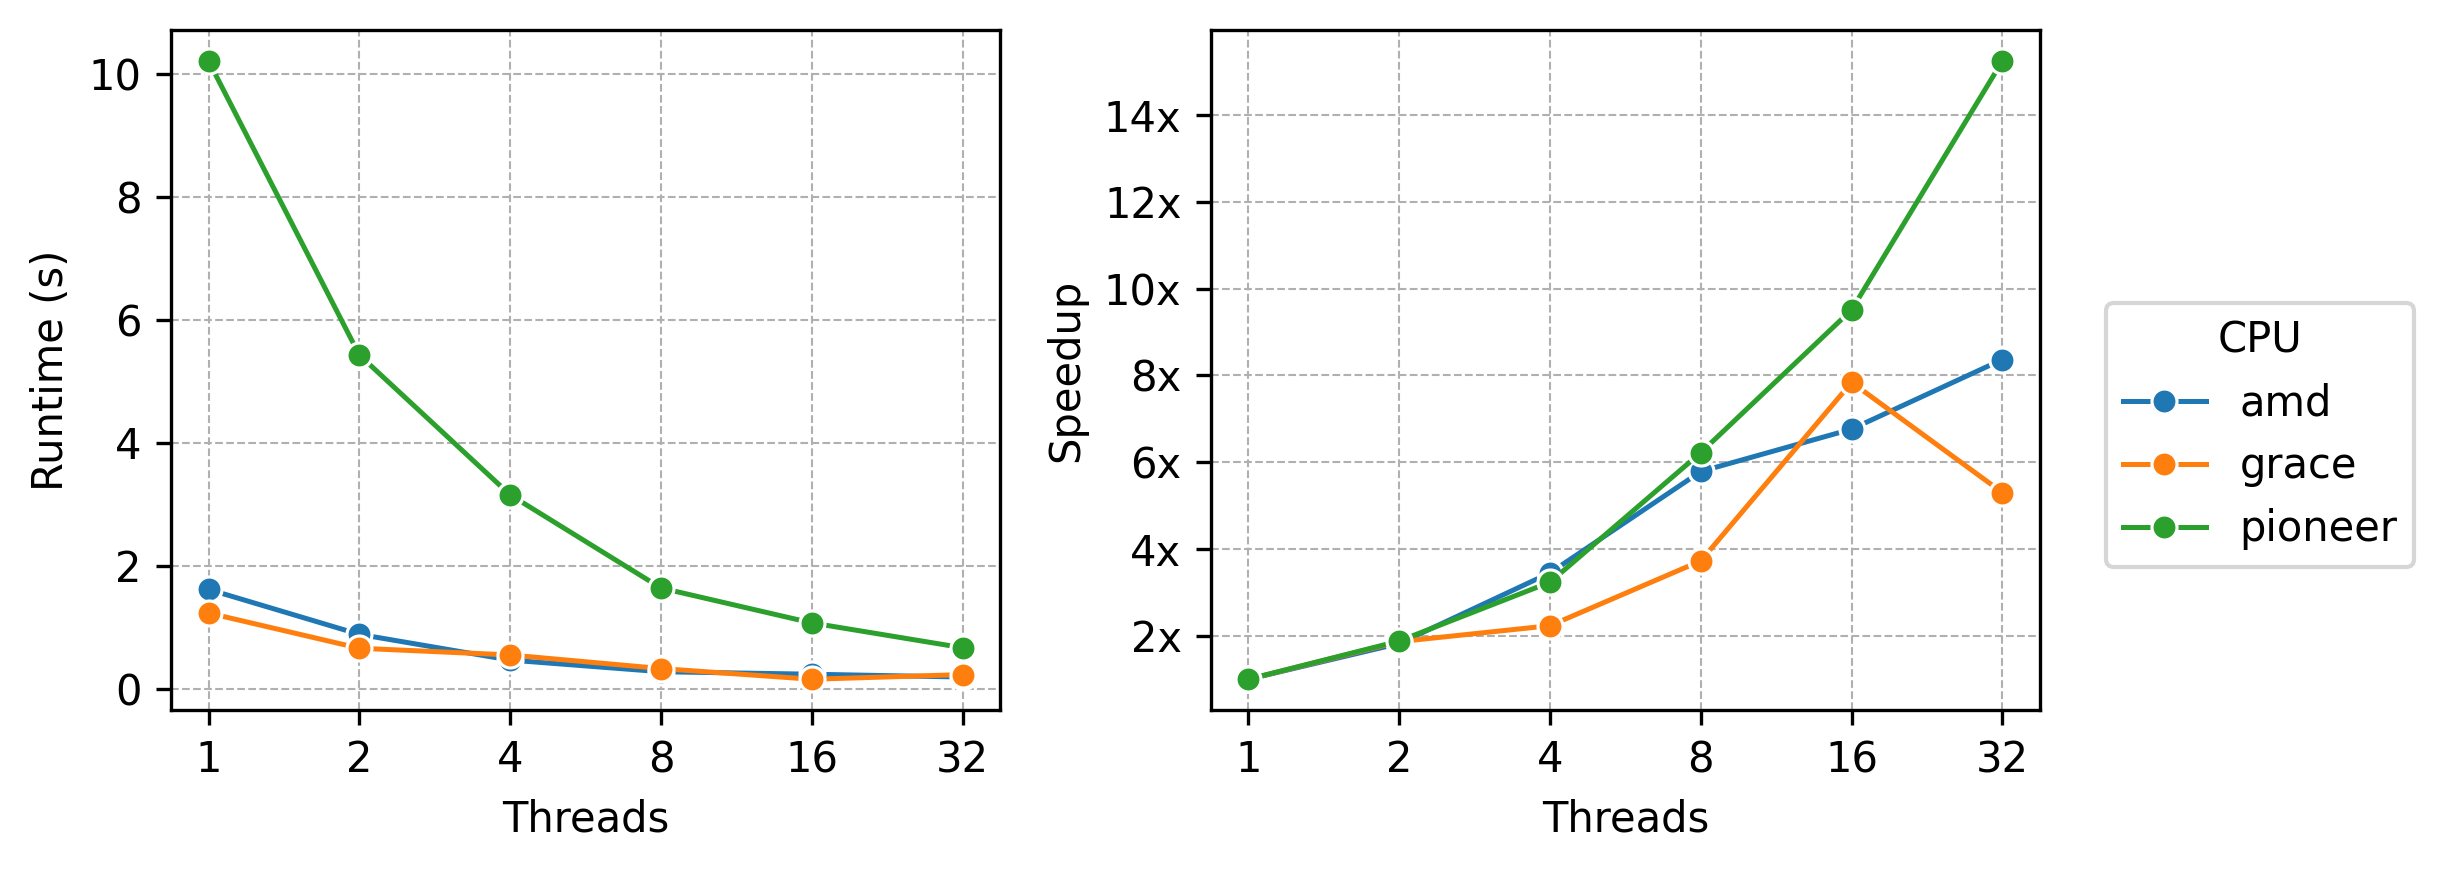
\includegraphics[width=0.95\linewidth]{images/other_platforms.png}
\caption{Strong scaling performance of the \texttt{pthreads} implementation on the \texttt{europe\_osm} graph across three different hardware platforms. The left panel shows the absolute average runtime in seconds. The right panel shows the corresponding speedup relative to the single-threaded performance on each respective platform.}
\label{fig:platform_comparison}
\end{figure}